\chapter{Results}
\todo{Overview}


\section{Proceeding} 
This section describes the proceeding how the results were achieved.

Following observations during research were made:
\begin{itemize}
	\item Every non metamodel based tool uses its own, specific approach for abstract language data structure transformation, validation, persistence and editing.
	\item In GMF, the \emph{Notation model} generically encapsulates the state of the visual representation. The \emph{Extensible Type Registry} determines a type or specialization type for which is used to guide Notation model element creation. Both 
	\item After short evaluation of MPS, the restrict usability of \emph{projectional textual is undesirable} for the intention of this thesis. This editing concept is template or form based, not free textual.
	\item The report \cite{Barista} about Barista shows the successful use of a variant of Harmonias incremental parsing algorithms in projectional editors to achieve \emph{stable abstract data structures}.
	\item Harmonias incremental parsing algorithm for GLR parsing requires the Parser to handle \emph{sentential forms}.
	\item Proxima uses a \emph{Structured Token for graphical presentation}, but does not allow it to be directly edited.  Its seven layer architecture with bidirectional model transformations between each allows high flexibility. Dependant layers especially regarding possible user interaction on different layers, with the complexity to maintain bidirectionality by two unidirectional transformations and updating instead of replacing model elements was considered undesirable. Several model transformation languages for EMF exist, so structural transformations are possible and separated if required. 
\end{itemize}

The Xtext framework was examined in respect of adding alternative representations and related problems. Following central perceptions were made:
\begin{itemize}
	\item Structure of textual representation is coupled to the structure of the model. This characteristic is condoned with reference to EMF model to model transformations.
	\item Used parsing technology results in unstable models. This characteristic is factored out until its impact on the solution in the discussion.
	\item The grammar must completely describe the model. 
	\item No isomorphism from grammar production to \code{EObject} exists, which means multiple representations of the same \code{EObject} are possible.
	\item The Parse Tree Constructor determines the production used for model to text transformation. Different textual representations already exist, but are not available. \\
\end{itemize}
 
 
The first improvement is to allow \emph{switchable textual representations}. This has been conceptually solved by extending the parse tree constructor and by providing a hint to guide the parse tree construction. A hint simply identifies the next production part.
The parse tree constructor is conceptually extended to
\begin{enumerate}
	\item determine all valid solutions for a node and assign them to it and
	\item to prefer certain hints while the resulting parse tree is constructed.
\end{enumerate}
For combined use with the parse tree constructor a Notation model was developed to
\begin{itemize}
	\item provide a proper place to assign alternative presentations and
	\item to uniquely identify productions or parts of it as hints.
\end{itemize}
To uniquely distinguish a specific tree construction for hints, the structure resembled a parse tree structure. The notation model was extended to substitute the parse tree accordingly.\\


\emph{Structured Tokens} highlighted the usage of nested structured data, like \code{EObject}s as Tokens. To integrate Structured Tokens in a textual serialization, a Structured Character concept was developed. It is based on the basic idea to use a private, unique character as a key for a map entry of a data structured persisted in an adjacent resource, like a file. The designated solution are UTF8 private use characters and a wrapping Lexer which resolves and types the \code{EObject}s from the adjacent resource. This enables the use of \code{EObject}s as atomic characters on the character stream. \\

The possibility to use \code{EObject} on the character stream enables the use of Notation model elements on it. Notation model elements represent parts of the Parse Tree or \emph{Sentential Forms}. To allow their use as \emph{Sentential Token} two improvements are necessary:
\begin{itemize}
	\item The extended Lexer must assign the Token name of the Sentential Token properly. The name can not be determined by the generic Notation model elements type, but by a general Notation Metamodel specific rule, which resolves the grammar relation of the Notation element.
	\item The input grammar for the used Parser generator must be post processed, so that each non terminal on the right hand side of a rule is replaced by an alternative. The alternative consists of the original non terminal or a terminal with the synthetic name of the grammar related element, which would be assigned by the Lexer.
\end{itemize}
Serialized Sentential Tokens are named \emph{Sentential Characters}. Sentential Characters alone simply hide the data structure of a production part in one character and perfectly integrate in the language described by the context free grammar grammar. \\

To improve the use \emph{Structured Characters} for Presentation, following enhancements are suggested:
\begin{itemize}
	\item Extensible Parse Tree Constructor, which optionally specializes the determined type based on additional constraints. This is similar to GMFs Extensible Type Registry.
	\item To omit Parse Tree construction, if a specialized presentation type was found. A graphical editor could then safely operate on the Language model elements.
\end{itemize}
A user interface could create a graphical editor at the place of his specific specialized presentation character and operate on the Language model elements it hides.\\


In discussion, the problem of unstable models and its impact on the suggested solution is resumed.


\section{XText Analysis}
This section analyses Xtext beyond the scope of Xtexts manual \cite{XTextMan}. At the beginning, isomorphism relations of Metamodel and grammar is discussed. Insights about isomorphism explain the variety of valid Parse Trees for a model. This leads to further insights in the Parse Tree Constructor. Subsequent peculiarities of Xtexts grammar are mentioned, followed by deficits of XtextResource and Xtexts Node Model for the desired solution.

\subsection{Model Grammar Isomorphism}
The explicit return types decouple the EObject type from the grammar rules in a well defined manner. Simple actions already made this possible, but the subtype of return type constraint strongly limited its useability. Return types raise the abstraction level, because an \code{EObject} of the abstract syntax can have a context dependent representation. It also allows multiple representations of the same EObject type, so this has a special significance for the Parse Tree Constructor.

On the other hand, this changes the time complexity of Parse Tree construction from $O(N)$ to $O(c^N)$ of the current XText implementation. The following explanation of choice mappings hint the problem, but it is explained in further detail in Parse Tree Constructor at \ref{sub:Xtxt:PTC}: 
\begin{xtxt}
Z 	:  "A" v=ID;
\end{xtxt}
this rule creates an \code{EClass} \code{Z} with an \code{EString} attribute \code{v}. Isomorphism is kept between the type \code{Z} and the production rule.
\begin{xtxt}
Z 	:  "A" v=ID  
	|  "B" n=INT;
	\end{xtxt}
creates an \code{EClass} \code{Z} with the attributes \code{v} of type \code{EString} and \code{n} of type \code{EInt}.  Isomorphism of the type to production rules is lost, but might be regained by a constraint if \code{v} or \code{n} is assigned. Isomorphism to a grammar rule is kept.
\begin{xtxt}
Z returns A : "A" v=ID;
Y returns A : "B" v=ID;
\end{xtxt}
No isomorphism of the type \code{A} to a grammar rule, because both rules return an \code{EObject} of type \code{A}.

\subsection{Parse Tree Constructor} \label{sub:Xtxt:PTC}

For example, if the following grammar parses \kode{somekeyword 0 C}:
\begin{xtxt}
S  	:  	v=A 
	| 	v=X;

A returns Obj	: 	l=B r=C   ;
X returns Obj	: 	l=Y r=Z   ;
B returns N  	:  	"somekeyword" 	v="0";
Y returns N  	: 	"otherkeyword" 	v="0";
C 		:  	 "C" ;
Z 		: 	 "Z" ;
\end{xtxt}
following AST will be constructed \todo{fix this} \\ 
      Obj			\\
     /   \textbackslash		\\
N(v='0')   C	\\
To create this parse tree without a node model, the decision if the rule of the root EObject is 'A' or 'X' can just be decided after determining the type of it's right child 'C'. \\

It is possible that all grammar rules return the same type, so type information would be useless to guide production rule resolution.\\


\subsection{Grammar}
In the XText grammar, it is not possible do statically assign a value  to a structural feature. For example to assigning \code{0} to an integer attribute \code{v} of class MyBoolean in the "false" case and \code{1} in the "true" case requires to write a special value converter. 
\begin{xtxt}
MyBoolean:  "true" | "false"
\end{xtxt}

A much greater impact on the grammar is it's inability to express left recursive grammars and the consequences. This is owed to the LL(*) parsing algorithm of ANTLR, the parser generator used by XText. This requires left factoring and grammar rewriting which lead to XText allowing tree rewriting of the AST by assigned actions. If only parser and AST construction is regarded, this is more or less an inconvenience for the grammar designer who needs to left-factorize, but it creates problems regarding parse tree construction and validation for XTexts current implementation. Considering that the current parse tree construction algorithm has a runtime of $O(c^N)$, it is arguable to use an GLR parsing algorithms with  $O(n^3)$ to avoid the need for grammar massaging and thus AST rewriting.

\subsection{XtextResource}
XText is, like EMFText \cite{EMFTextMan}, integrated in EMF as an EMF Resource. The responsibility of resources is to serialize and deserialize models, this leads to various problems: 

\begin{itemize}
	\item The grammar must describe the whole model: the model must not contain non volatile information which is not regarded by the grammar. Adding additional information, like an ID, is impossible without incorporating it in the grammar. To circumvent the restriction that the whole model must be textually described. A possible solution would be to create additional EObjects in an additional Resource, which points at the EObject in the XTextResource which should be enriched. With an ECrossReferenceAdapter the inverse references and thus the additional information of the extended object. This technique to extend an EObject in a non invasive manner is used to implement UML2 stereotypes in eclipse UML. This concept depends on references and their integrity.
	\item The XText editor edits the text file, meaning it edits the serialized form of the model, not the model. In conjunction with a non incremental parser, model elements are replaced instead of updated. Furthermore, EMFs ResourceSet which keeps referential integrity is bypassed. XTexts demands the programmer to handle referential integrity or to "return stable fragments for its contained elements ". For example the expression "int i=0" in a programming language does not contain an intrinsic identifier, so this is impossible for an arbitrary language. UML2 solves the problem of referential integrity by assigning every model element an universal unique identifier (UUID). These UUIDs are handled by the resource and are  externally attached to the model objects. To keep referential integrity, either modifications must be done in a ResourceSet or extrinsic UUIDs must be used. 
	\item Because the model contained in a resource is \todo{wrong!} not modified in a ResourceSet and extrinsic, non grammar conform information like IDs can not be added or integrated persistently to model elements referential integrity can not be maintained. On the other hand to determine changes to update a model without unique IDs are based on heuristics, thus potentially inaccurate.  To enable proper updates and keep referential integrity, editing must not be done on the textual serialized form of a model. This does not contradict to store the model in textual form for e.g. viewing and versioning. 
\end{itemize}

\subsection{Node Model}
The potential use of the node model is strongly restricted in Xtext, for the following reasons:
\begin{itemize}
	\item the node model is not an EMF model. 
	\item The node model is not explicitly available without running the XText parser, because it is created by the parser from information of the concrete serialized language model. 
	\item The use of the runtime instances of the node model is restricted by the API: ``clients should never keep a reference to a node as it may be invalidated at any time and the very same object could be reused in another subtree of the full parse tree.''\cite{XTextAPI}
	\item The node model is not updated during parse tree construction. If an update is required, an additional parse with its problematic replacing instead of updating behavior is necessary.
	\item Even if the parse tree constructor would construct the node model, it takes the first valid solution. It is not possible to choose between different valid representations or prefer a valid one which are semantically equivalent, e.g.
\begin{xtxt}
Foreach 		: 	Map | For;
Map returns FE  	:  	"map" 		v=ID;
For returns FE  	: 	"foreach"	v=ID;
\end{xtxt}
\end{itemize}


\section{Outline Solution}
% Outline Solution
The general idea of the presented solution combines three simple concepts. The first two following points already allow to operate on the parse tree part in the map:
\begin{itemize}
	\item The use of private characters as a unique key for a map. The value of the map is an object, thus a single character can be resolved to an arbitrary data structure.
	\item The parse tree is a tree data structure. If a part of the tree produced by a token sequence is saved in a single token, that token is a valid substitute for that part of the tree.
	\item A parse tree constructor, which constructs a parse tree from an abstract syntax tree and is extensible with regard to assign types to and to skip parse tree construction for invisible elements. This allows the graphical editor to use the abstract syntax tree directly as data source. 
\end{itemize}

Figure \ref{ConceptFigure} shows the conceptional overview. \todo{IntegratE}

\begin{figure}
\centering
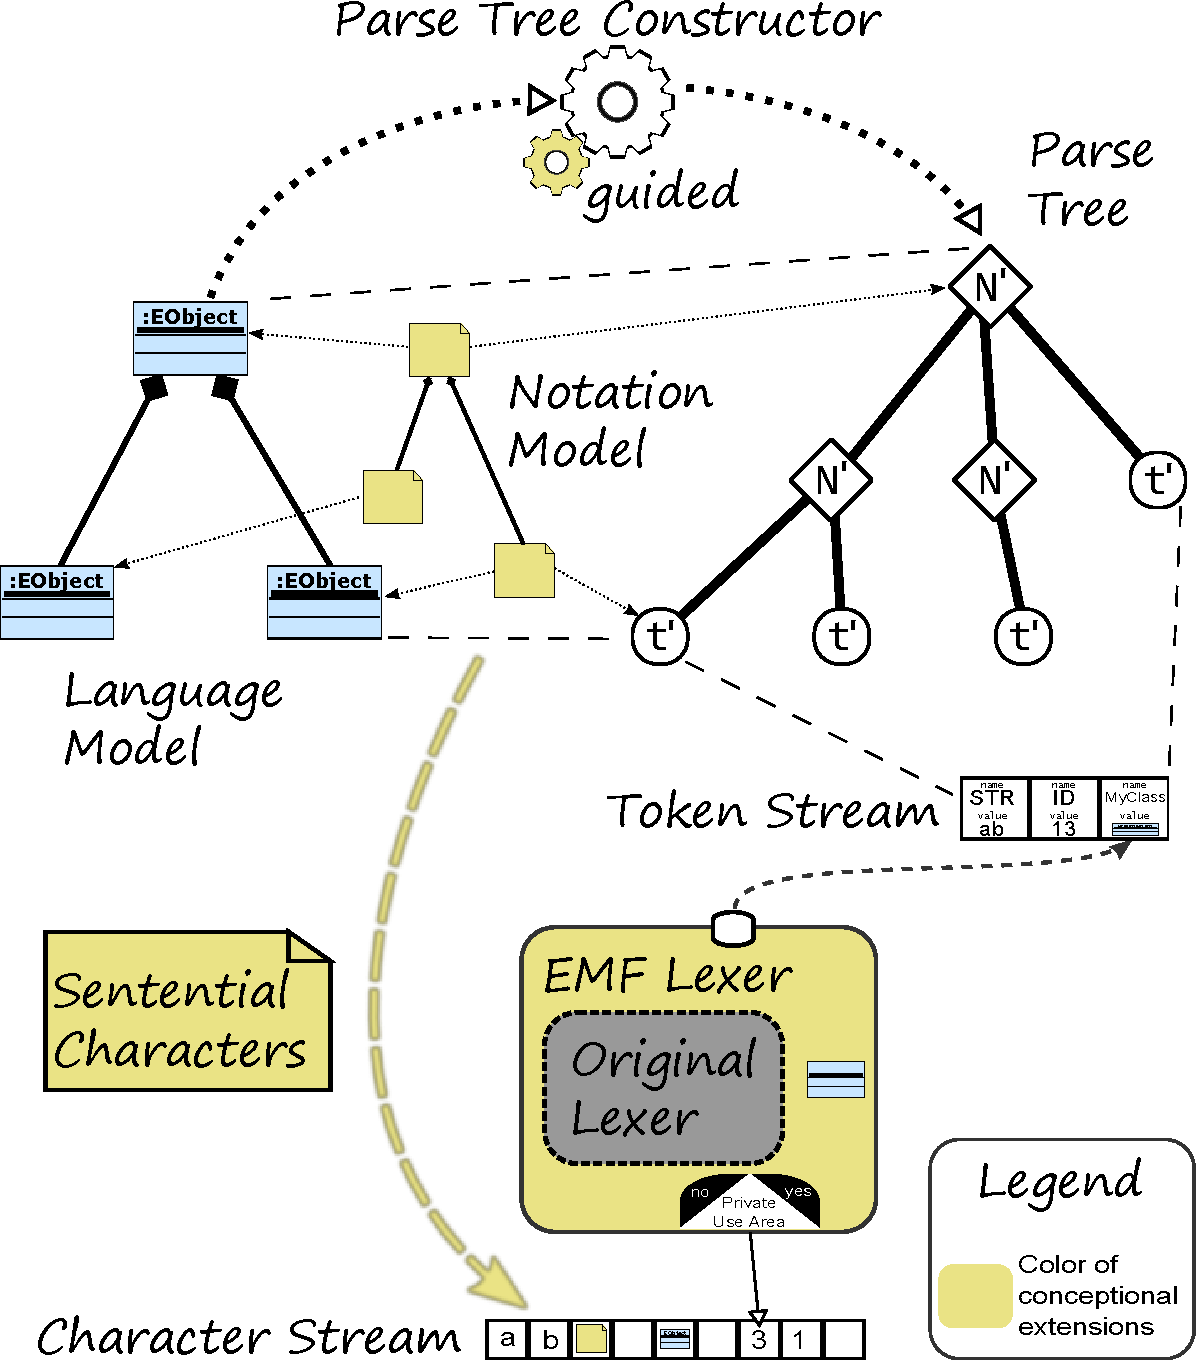
\includegraphics[scale=0.75]{gfx/ex/Concept} 
\caption{Conceptual Overview}
\label{ConceptFigure}
\end{figure}

On the right side of the diagram are the classical parser related elements, from below upwards:
\begin{itemize}
	\item a character stream
	\item a lexical analyzer or ``Lexer'', which reads the characters and groups them into Tokens.
	\item the token stream, which is produced by a Lexer and used by a Parser to create the ``Parse Tree''
\end{itemize}

On the left side is a ``Language Model'', which is deduced from the Parse Tree by the attribution of the grammar. In parser literature, \emph{this Language Model is called Abstract Syntax Tree}. The use of a modeling term instead of parsing term emphasizes where models are integrated and that a language description in modeling concepts is abstract. In contrast to context free grammars a language in modeling terms lacks a concrete notation. It is not mandatory that the language model is equal to the abstract syntax tree. Until both data structured are combined in \ref{sec:MM:CFGs} \todo{check ref}, both terms are used. \\
The inverse transformation, from Language Model to Parse Tree is done by the Parse Tree Constructor. This transformation is ambiguous, because for one Language Model more than one valid Parse Tree can be constructed. \\
This described architecture is implemented in XText. This thesis conceptually extends the architecture by extending the Parse Tree Constructor, by the introduction of a ``Notation Model'' and an ``EMF Lexer''.\\
The Parse Tree Constructor is extended by 
\begin{itemize}
	\item adding valid alternative constructions to the Notation Model and regarding them while constructing the Parse Tree. 
	\item extensible rule evaluation capability to further specialize production parts depending on constraints.
	\item omitting Parse Tree branch construction for decorated Notation Model elements.
\end{itemize}
The Notation Model is introduced to:
\begin{itemize}
	\item be a serializable model
	\item to add an approved design of graphical editors to separating language elements and their corresponding notation state.
	\item to guide the Parse Tree constructor to be able to unambiguously construct a certain Parse Tree. This lead to a model with nearly the same expressive power as the Parse Tree itself, so the Notation Model was slightly extended to \emph{substitute the Parse Tree}. Figure \ref{ConceptFigure} shows the Notation Model separated from the Parse Tree as a bridge between Language Model and Parse Tree because this integration feature is the advantage of the Notation Model over the Parse Tree. The degree of overlapping functionality of Notation Model and Parse Tree did not justify separated data structures.
\end{itemize} 
The EMF Lexer is introduced to:
\begin{itemize}
	\item separate private use characters from the character stream used for the original Lexer.
	\item resolve the data structure identified by a private use character.
	\item determine a token name by properties of the \code{EObject}s in that data structure. This assignment process can be customized by additional rules that traverse the resolved data structure.
\end{itemize}










\section{Guided Parse Tree Constructor}
The Guided Parse Tree Constructor is responsible to find all valid parse trees for the current language model and select the best tree. The actual Parse Tree construction process is twofold:
\begin{itemize}
	\item find all combinations of production rule applications that uniquely distinguish valid words and
	\item create a parse tree according to the most promising combination. 
\end{itemize}
 
The suggested solution is close the one implemented in Xtext. Xtexts solution, which is described in \ref{xtxt:ptc}, stops after finding one combination. 
To enable multiple representations, the alternatives need to be made available. This is done by the notation model, which is described in \ref{chp:NotMM}. The notation model is able to be equivalent to a parse tree, but also allows to refer to following productions, called hints. EMFs \code{ECrossReferenceAdapter} virtually creates bidirectional references from unidirectional ones. This allows the use or reuse of notation model elements which refer to AST nodes just by getting all referring \code{EObject}s and filtering a type.

\todo{blueprints based on s-attributes. Tree struct based on SAttrs.}

\paragraph{Hints}
A hint is a reference to a following production. So with hints, a node in the parse tree is not only labeled by its non terminal, but also by its production. Hints specify a single production without referring to a parse tree part, which is important, if multiple productions are possible. Thus, hints do not refer to actual content but define the structure of the content. Regarding the Parse Tree Constructor, the AST is present, but it is ambiguous which structure to use to hold its contained data.  

\paragraph{Parse Tree Construction Steps}
The basic steps of Parse Tree Construction are:
\begin{enumerate}
	\item compute all possible solutions. This results in a forest of parse tree blueprints.
	\item determine the best tree. Which criteria compose the best tree are explained below.
	\item produce a parse tree for the best tree. 
	\item compress the forest. For each branch which branches the best tree, set the first node of the branch as an alternative representation of the best trees node it branches from.\\
\end{enumerate}

\paragraph{Ranking criteria} Criteria that determine the result tree are ranked from most to least important:
\begin{enumerate}
	\item Use notation model hints, if exits. Hints are likely set by the user and thus have top priority.
	\item Number of similar productions to the previous parse or parse tree construction state, which is saved in the notation model. \todo{xxx }Keeps stable.
	\item User preferences.
	\item Language designer preferences.
	\item Number of default values used as negative criteria.
	\item Number of direct EObjects required as negative criteria.
\end{enumerate}

\todo{blueprints 2 parsetree}

The suggested behavior is, that the user does not specify the whole alternative representation, but selects an alternative, let the Parse Tree Constructor create and display the new representation and iteratively refines the presentation. 


\section{Grammar}
In this section, a metamodel for an synthesized attributed grammar is developed to formally describe the required grammar relation of the Notation Metamodel. The described grammar is simpler than Xtexts grammar, especially in regard to Actions. First a Metamodel for a normal, non attributed, grammar is defined, then an example instance of it is presented, finally the grammar metamodel is completed by an attribution extension.

\subsection{Grammar Metamodel}
%%%%%%%% GrammarMM	%%%%%%%%%%%%%%%%%%%%%%%%%%%%%%
\begin{figure}
\centering
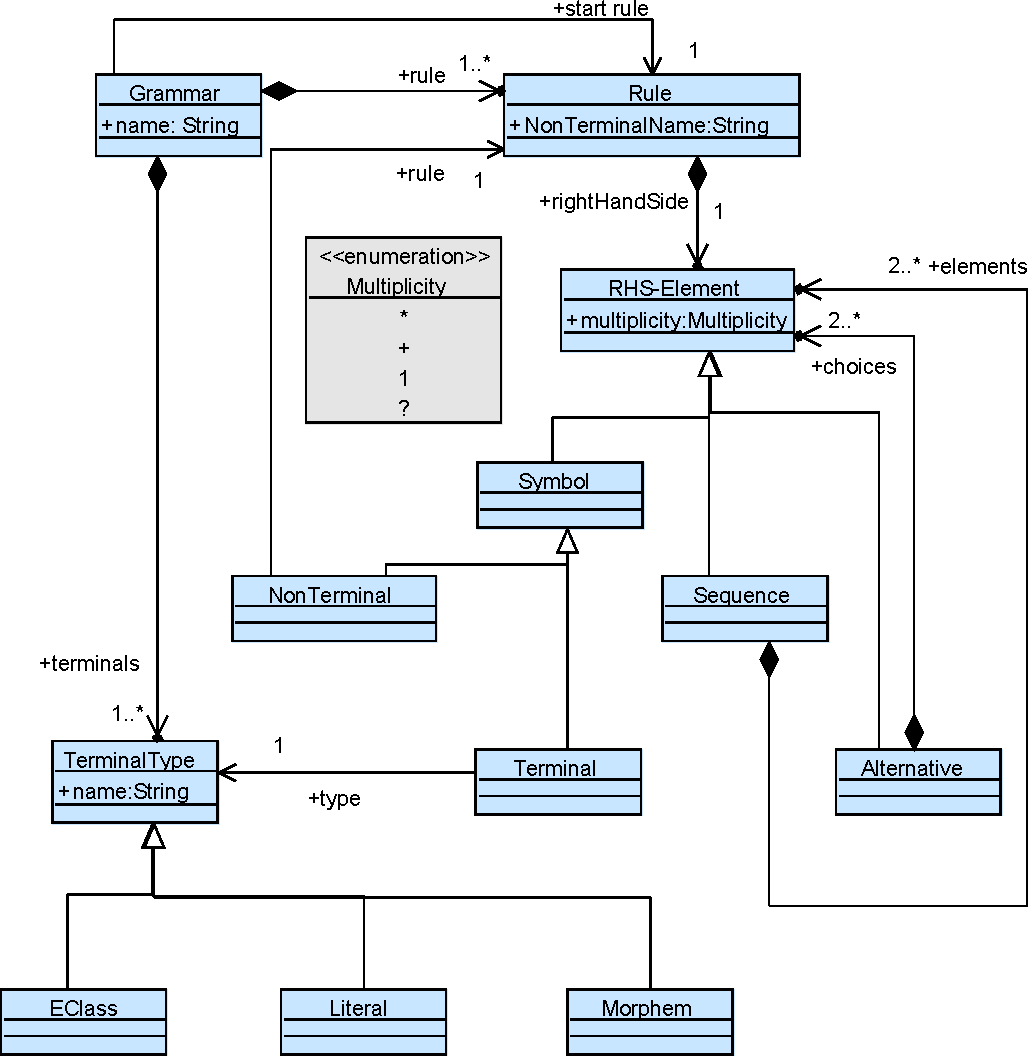
\includegraphics[scale=0.85]{gfx/ex/Grammar_CFG} 
\caption{EBNF Grammar Metamodel}
\label{MM:EBNF}
\end{figure}

Figure \ref{MM:EBNF} shows a metamodel for an EBNF grammar. The metamodel lacks the ability to define lexemes.  \\
Compared to the definition of a context free grammar, the non terminals are the set of \code{NonTerminalName}s of \code{Rule}, the terminals are the set of \code{name}s of \code{TerminalType}, the start symbol is the \code{Rule} referred by \code{Grammar} and the productions are implicit described by the directly and indirectly contained elements of the \code{Rule}s. The \code{NonTerminal} and \code{Terminal} elements in the grammar are just references to the real non terminals and terminals. This definition overlap is owed to the fact that the same terminal may appear multiple times in productions, which must be distinguishable . The denomination allows for example in following rule to be \code{b$_1$} an instance of \code{Terminal}, \code{C} and instance of \code{NonTerminal} and \code{b$_2$} another instance of \code{Terminal}, but referring to the same \code{TerminalType}:
\\\begin{code}
A : b$_1$ C b$_2$
\end{code}\\

The \code{Grammar} has at least one \code{Rule} and one \code{TerminalType}. The \code{Grammar} has exactly one \code{start rule}. The \code{Rule}s have a name and contain exactly one element as their \code{rightHandSide}. This element might be either a \code{NonTerminal}, a \code{Terminal}, a \code{Sequence} or an \code{Alternative}. \code{Sequence}s and \code{Alternative}s are containers for at least two \code{RHS-Element}s. \code{Sequence} are \code{a b c} or \code{(a b)+} for example. \code{Terminal} and \code{NonTerminal} hold references to their unique type they represent. \code{Symbol} just provides abstraction but does not add expressivity to the language itself. Every \code{RHS-Element} has a \code{Multiplicity}, so exactly one \code{1}, one or none \code{?}, zero or more \code{+} or any multiplicity \code{*} can be expressed. Subclasses of \code{TerminalType} are present to allow a more detailed specification of \code{TerminalType} in later models.


%%%%%% GrammarMM()	%%%%%%%%%%%%%%%%%%%%%%%%%%%%%%

%% Grammar Instance
\subsection{Grammar Example}
\begin{figure}
\centering
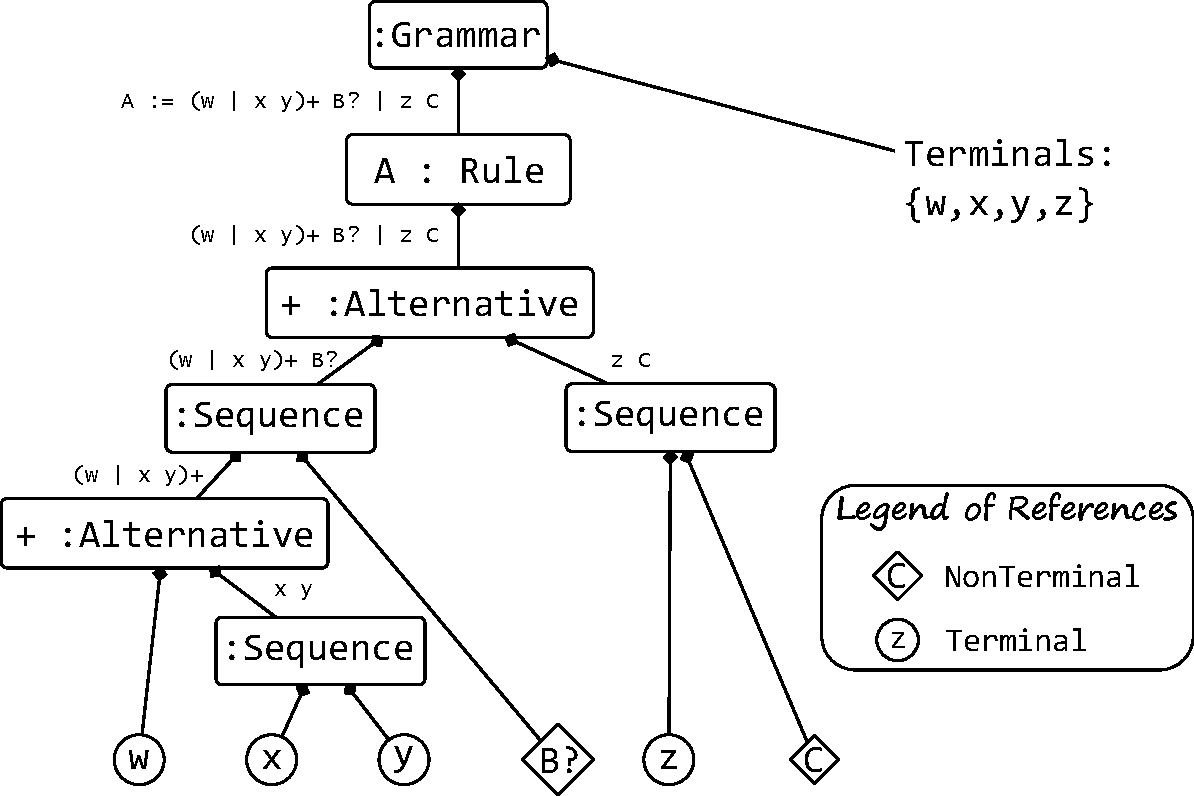
\includegraphics[scale=0.7]{gfx/ex/grammarExample} 
\caption{Example Rule ``A := (w |x y)+ B? | z C''}
\label{MM:GrammarExample}
\end{figure}
Figure \ref{MM:GrammarExample} shows the model instance of the EBNF metamodel \ref{MM:EBNF} of the grammar  \code{A := (w |x y)+ B? | z C}. The grammar rules \code{B} and \code{C} are left out, as well as the start rule reference. The references to the symbols \code{w}, \code{x}, \code{y} and \code{z} are replaced with the name of the referenced symbol.

\subsection{Attributed Grammar}
\begin{figure}
\centering
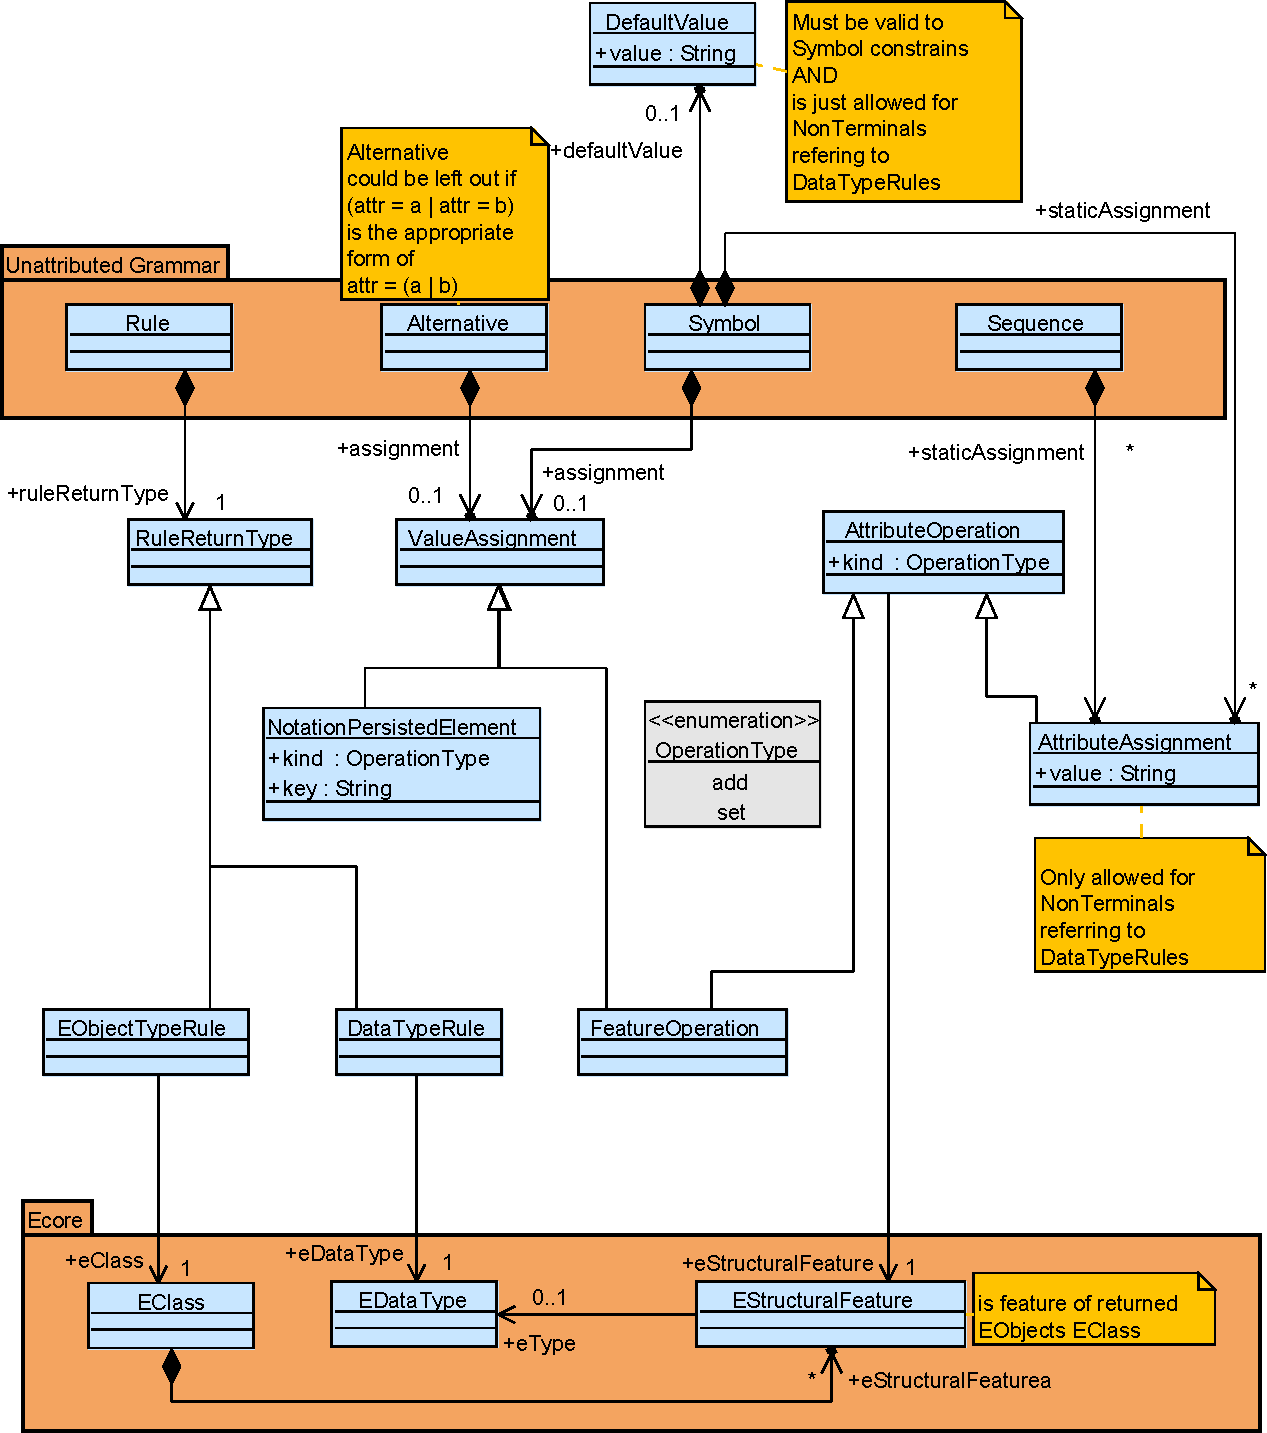
\includegraphics[scale=0.7]{gfx/ex/Grammar_Attributed} 
\caption{Attributed Grammar metamodel extension}
\label{MM:AEBNF}
\end{figure}

The metamodel defined in \ref{MM:AEBNF} adds attribution and default values to the grammar. It uses metaclasses from the metamodel \ref{MM:EBNF} for context free grammars. The packaging is for documentation purpose only, because the metaclasses of the CFG metamodel refer to the current metaclasses. \\
Each \code{Rule} has a \code{RuleReturnType}, which might be an \code{EClass}, if it is a an \code{EObject} returning rule or an \code{EDataType}, if it is a Data Type Rule. The additionally distinction in \code{EObjectTypeRule} and \code{DataTypeRule} is for presentation purposes only, this makes it obvious in the diagram when an \code{EObjectTypeRule} is used. For a real implementation a reference from \code{Rule} to an \code{EClassifier} would be sufficient. \code{EClassifier} is the supertype of \code{EClass} and \code{EDataType}. \code{Symbol} now can contain a  \code{defaultValue}, which is a \code{String}.  \code{String}s are structureless, so the use of \code{DefaultValue}s is restricted to  \code{NonTerminal}s referring \code{DataTypeRule}s and  \code{Terminal}s only. The  \code{String} must not violate the  \code{Symbol}s constraints. Given the example \code{attribute+=TerminalSymbol}, an attribute assignment is realized by \code{TerminalSymbol} containing a  \code{FeatureOperation} with \code{kind} set to  \code{add} and a reference to the  \code{EStructuralFeature} named \code{attribute}. The \code{EStructuralFeature} must be contained in the  \code{EClass} of the returned \code{EObject}s type. In contrast to Xtext, it is possible to assign statically a structureless value to an attribute, for example 
\begin{xtxt}
Rule : {ruleAttribute="true"} "1"
\end{xtxt}   
which means that if the rule matches \code{ruleAttribute} is assigned to \code{"true"}. This can be done for an arbitrary amount of \code{EStructuralFeatures}. \code{NotationPersistedElement} allows to persist a String in the notation model, this allows to share data between \code{Alternatives}. \\
\code{Alternatives} also contain a \code{ValueAssignment}. This could be omitted if 
\begin{xtxt}
attribute= (a | B)
\end{xtxt}
would not be allowed and instead only the alternative 
\begin{xtxt}
(attribute = a | attribute = B)
\end{xtxt}
would be allowed.
%% Grammar Instance()